\section{Applying the C2W model}

\subsection{Language Modeling}
\label{subsec:language-model-c2w}

In this section we use the C2W model and a recurrent LSTM to perform language modeling as 
described in~\cite{DBLP:journals/corr/LingLMAADBT15}.
The neural network is going to compute the $\log$ propability $\log[ p(\mathit{w}) ]$ of the 
sentence $\mathit{w} = w_1, \dots, w_m$. As previously discussed in section~\ref{sec:language-modeling} this can be 
decomposed into the sum of the conditional log probabilities $log[ p(w_1,\dots,w_m) ] = \sum_{i=1}^{m} log[ p(w_i | w_1,\dots,w_{i-1}) ]$.
This model will compose the previously described word representations of $w_1,\dots,w_{i-1}$ to compute 
$log[ p(w_i | w_1,\dots,w_{i-1}) ]$ using a LSTM unit.
The model is shown in figure~\ref{fig:c2w-language-model}. The first stage can use either the embeddings generated with the C2W model
$f(w_i) = e_{w_i}^C $ or simply word lookup tables $e_{w_i}^W = P * 1_{w_i}$.

Every time we input a new word $w_i$ from the sequence we get the LSTM state $s_i$. The state $s_i$ is then used to predict word $w_{i+1}$.
The state $s_i$ is projected into a vector of size $|V|$ (the vocabulary size). The softmax is a $d \times V$ table, 
which encodes the likelihood of every word type in the vocabulary in a given context. 
The softmax layer will ensure a valid log probability distribution. This way we can choose the word type with the maximal likelihood.
Maximizing the conditional log-likelihoods during training will improve the modeling 
of $p(\mathit{w})$~\cite{DBLP:conf/interspeech/MikolovKBCK10}.
More details regarding the softmax layer are explained in section~\ref{subsec:softmax}.

\begin{figure}[H]
\begin{center}
  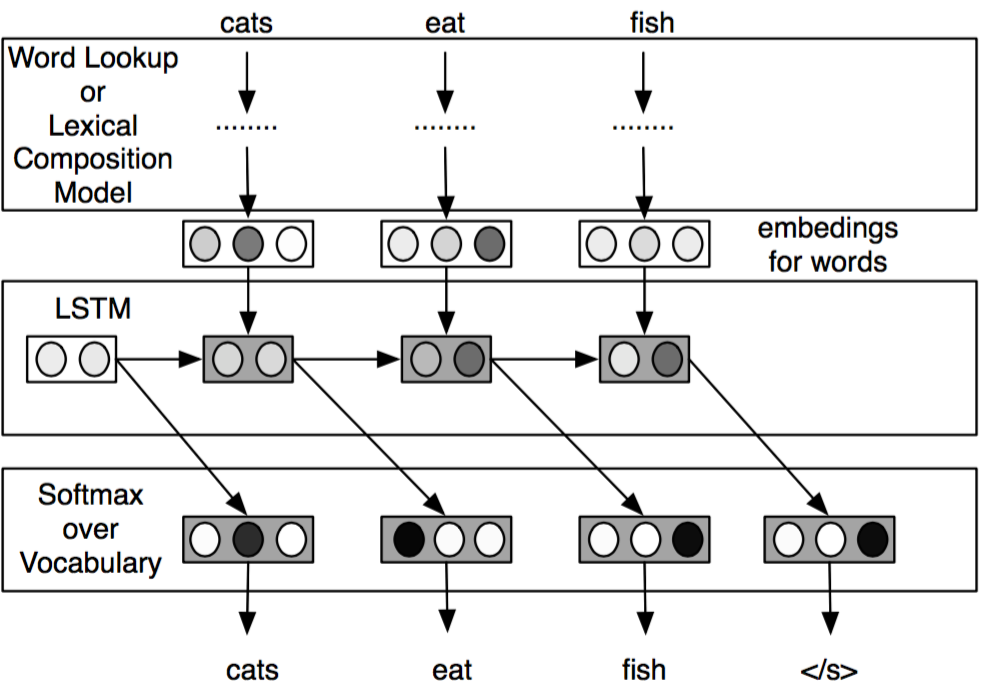
\includegraphics[width=0.6\textwidth]{./img/c2w-language-model}
  \caption{Neural network for language model. The C2W model is at the top, the word embeddings are then fed into an recurrent LSTM.}
  \label{fig:c2w-language-model}
\end{center}
\end{figure}


\subsubsection{Evaluation}

The original paper~\cite{DBLP:journals/corr/LingLMAADBT15} compares the performance of the language model 
in terms of it's perplexity~\ref{subsec:perplexity}. To minimize the perplexity value means to have a better fitting language model.
Perplexity cannot be used to compare models with different vocabularies,
since there are fewer outcomes in the softmax, the global perplexity can decrease.

\begin{table}
\begin{center}
\begin{tabular}{ l l l l l l }
  \hline
             & \multicolumn{3}{|c|}{Fusional} &   \multicolumn{2}{|c|}{Agglutinative} \\ \hline
  Perplexity   & English & Portugese & Catalan & German & Turkish \\
  %5-gram KN    & 70.72   & 58.73     &   39.83 & 59.07  & 52.87   \\
  Word Lookup  & 59.38   & 46.17     &   35.34 & 43.02  & 44.01   \\
  C2W Model    & 57.39   & 40.92     &   34.92 & 41.94  & 32.88   \\
  \#Parameters  &         &           &         &        &         \\
  Word Lookup  & 4.3M    & 4.2M      &  4.3M   & 6.3M   & 5.7M   \\
  C2W Model    & 180K    & 178K      &  182K   & 183K   & 174K   \\

\end{tabular}
\end{center}
\caption{Perplexities of different language models and the test configuration (From~\cite{DBLP:journals/corr/LingLMAADBT15}).}
\label{tab:perplexity}
\end{table}

In table~\ref{tab:perplexity} the perplexities and the parameter counts are displayed for different language models.
The language model performance is tested on English, Portuguese, Catalan, German and Turkish; the data is extracted from wikipedia.
Every word embedding $e_{w} \in \mathbb{R}^{d_w}$ is going to have $d_w = 50$ parameters.
Therefore the model which uses a lookup table of word embeddings, contains at least $d_w \times |V|$ parameters.
The parameter count for the language model using C2W based embeddings depends on a few things. The number of parameters for each character
representation $d_C = 50$, and the number of parameters $d_{CS} = 150$ in the LSTM state $s_i$. The C2W model contains 8 matrices of 
size $d_{CS} \times d_C + 2d_{CS}$ (One for each of the 4 decision gates in both LSTM's). Additionally there is the character lookup table 
which has an entry for every character in the language $d_C \times |C|$. For English and 618 this works out to $15000 + 30900$ parameters.

\subsubsection{Nonce Words}

One feature of the C2W model is the ability to handle \textbf{nonce words}. These are words which do not occur in
any standard vocabulary, because they are created for use in a single occasion.
Because the C2W model doesn't rely on fixed tables of parameters, it can generate embeddings for these words.
This allieviates the need for OOV tokens for words not in the vocabulary (at least at the level of the C2W model).
In table~\ref{tab:nonce} we can see two nonce words and the 6 words which had the most similar word embedding
from the training vocabulary. As it is easily noticeable, the words intuitively seem of similar to the lookup word. 
This should be the intended effect, as this is more similar to human abilities.

\begin{table}
\centering
\begin{tabular}{ c | c }
   Noahshire &  phding \\ \hline
   Nottinghamshire & mixing \\
   Bucharest & modelling \\
   Saxony & styling \\
   Johannesburg & blaming \\
   Gloucestershire & christening \\
\end{tabular}
\caption{Nonce words and their most similar words from the vocabulary~\cite{DBLP:journals/corr/LingLMAADBT15}.}
\label{tab:nonce}
\end{table}


% ==========================================================================================
\subsection{Part-of-Speech Tagging}

Part-of-Speech tagging is the process of labeling words as corresponding to a particular part of speech. A simple tagging would be
to identify words as nouns, verbs, adjectives, adverbs, etc.
The model receives a number of words $w_1,\dots,w_m$ as input, and transforms them into word embeddings. These embeddings are then processed
in a bidirectional LSTM layer, just as described in section~\ref{subsec:bidir-rnn}. 
In contrast to the combining layer of the C2W model, we don't just use the final state of the LSTM output states, but all states.
The forward states $s^f_0,\dots,s^f_m$ and the backward states  $s^n_m,\dots,s^b_0$ are combined with  $l_i = \tanh(L^f s_i^f + L^b s^b_i + b_l)$.
Where $L^f$, $L^b$, $b_l$ are the parameters of the combining layer. The output label for each word $w_i$ is then obtained from a softmax layer over
all word labels.

\begin{figure}[H]
\begin{center}
  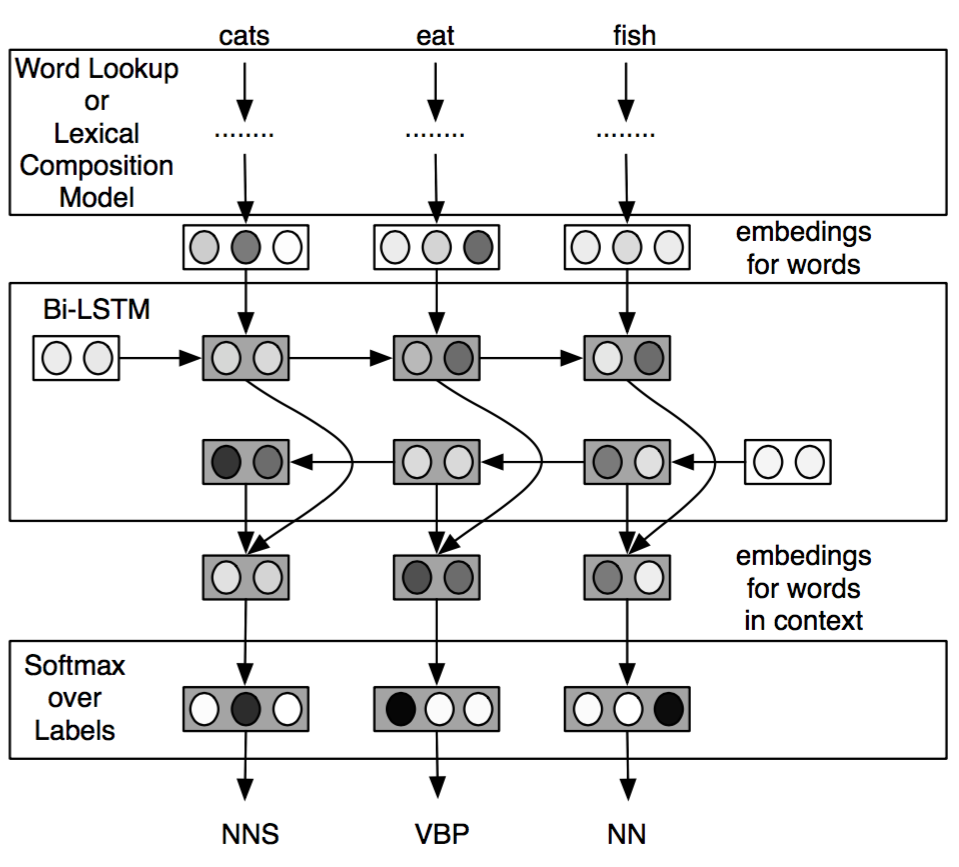
\includegraphics[width=0.6\textwidth]{./img/part-of-speech}
  \caption{The arhitecture of the NN for part-of-speech tagging (From~\cite{DBLP:journals/corr/LingLMAADBT15}).}
  \label{fig:part-of-speech}
\end{center}
\end{figure}

\subsubsection{Evaluation}

The POS tagging is evaluated on the same languages as before. We compare the POS model with word embeddings from a lookup table
as well as Stanford’s POS tagger with the C2W based POS tagger.
\begin{table}
\begin{center}
\begin{tabular}{ l l l l l l }
  \hline
  System       & \multicolumn{3}{|c|}{Fusional} &   \multicolumn{2}{|c|}{Agglutinative} \\ \hline
               & English & Portugese & Catalan & German & Turkish \\
  %5-gram KN    & 70.72   & 58.73     &   39.83 & 59.07  & 52.87   \\
  Word Lookup  & 96.97   & 95.67     &  98.09  & 97.51  & 83.43   \\
  C2W Model    & 97.36   & 97.47     &  98.92  & 98.08  & 91.59   \\
  Stanford     & 97.32   & 97.54     &  98.76  & 97.92  & 87.31  \\

\end{tabular}
\end{center}
\caption{Accuracy of the POS tagging in percent (From~\cite{DBLP:journals/corr/LingLMAADBT15}).}
\label{tab:pos-eval}
\end{table}


% ==========================================================================================
\subsection{Morphological inflection generation} 

Another application of C2W like model beyond language modeling is the morphological inflection generation~\cite{DBLP:journals/corr/FaruquiTND15}.
The goal is to perform a lingustic transformation some examples of the inflections which this model seeks to 
generate can be seen in table~\ref{tab:inflections}.
This model uses a neural encoder-decoder structure to generate the desired inflected output word.

The encoder part the model is virtually identical to the C2W model: 
Each word $w$ is broken up into it's characters $e_{c_1}, \dots, e_{c_m}$.
Then a bidirectional LSTM layer is used and th result is composed into the embedding $e$.

\begin{figure}[H]
\begin{center}
  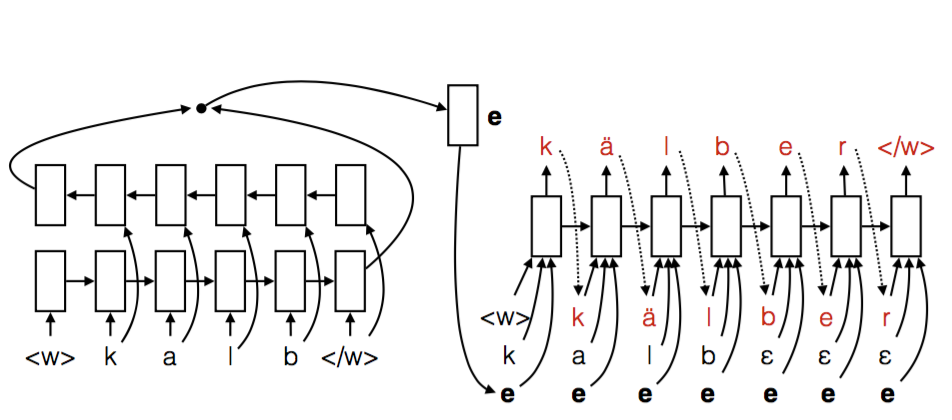
\includegraphics[width=\textwidth]{./img/inflection-generation}
  \caption{A endoder decoder structure for inflection generation}
  \label{fig:inflection-generatior}
\end{center}
\end{figure}

\subsubsection{Decoder}
This is a LSTM unit which will sequentially receive the word characters as input combined with the previous output and the word vector.
Every output state is computed as $s_t = g(s_{t-1}, \{e, y_{t-1}, x_t\})$. Where $g$ is the decoder LSTM unit,
$s_t$ is the LSTM output, $y_{t-1}$ the actual character output and $x_t$ is the current input character.
Since the input word might be shorter than the output, onece the input sequence runs out of characters we feed in an $\epsilon$ character
indicating null input: $x_t = \epsilon$. The vector representation for the $\epsilon$ character is learned just like any 
other character embedding in the C2W model.
The decoder decides to stop by outputting the word end token "$<$/w$>$".

\begin{table}
\begin{center}
\begin{tabular}{ l l l l }
  \hline
             & singular & plural \\ \hline
  nominative & Kalb & K\"alber \\
  accusative & Kalb & K\"alber \\
  dative & Kalb & K\"albern \\
  genitive & Kalbes & K\"alber \\
\end{tabular}
\end{center}
\caption{Example of an inflection table for the word Kalb (calf, German).}
\label{tab:inflections}
\end{table}

\subsubsection{Evaluation}

\begin{figure}[H]
\begin{center}
  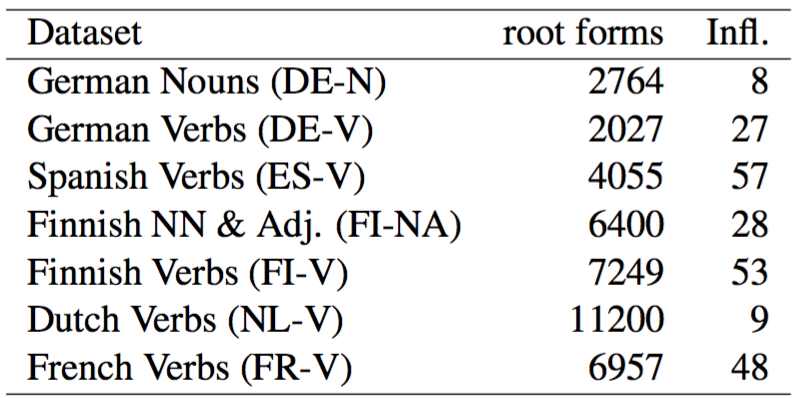
\includegraphics[width=.5\linewidth]{../slides/images/data_inflections}
  \caption{Languages for the POS-tagging evaluation~\cite{DBLP:journals/corr/FaruquiTND15}.}
  \label{fig:inflection-languages}
\end{center}
\end{figure}

The languages shown in figure~\ref{fig:inflection-languages} with
development and test sets containing about 200 inflection tables each.
The data was published by
\begin{itemize}
\item {[}Durrett and DeNero 2013{]} containing inflections for German, Finnish and Spanish.
\item {[}Nicolai et al., 2015{]} adding dutch and french to this dataset.
\end{itemize}

The results printed in table~\ref{fig:inflection-languages} are according to the original paper
comparable or better than other state of the art approaches. On average the results are better.
The main take-away is that these results were achieved without additional feature engineering. 
The model usually performed better than the other approaches, when the evaluation was performed on datasets with large training set.
\begin{figure}[H]
\begin{center}
  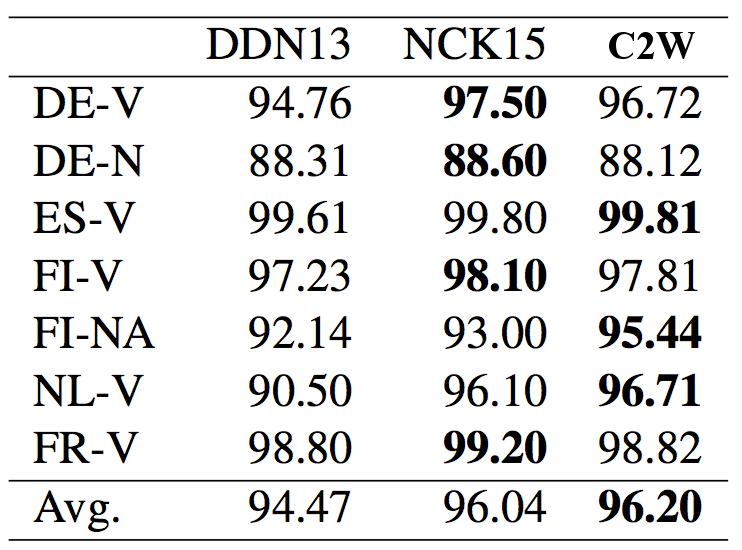
\includegraphics[width=.4\linewidth]{../slides/images/evaluation_inflections}
  \caption{Results for Languages from table~\ref{fig:inflection-languages}.}
  \label{fig:inflection-eval}
\end{center}
\end{figure}

% Comparison of current LSTMs based word embeddings with the character based method from Santos et al. \cite{DBLP:conf/icml/2014}